\subsection{Safety officer radio}
The safety officers do not interact directly with the AAs during an ongoing mission, but intervene in certain events. During these events it is crucial that voice communication is established between these two groups. For this purpose, the safety officers use a Motorola Mototrbo SL 2600 handheld radio with the same antenna and lithium-ion battery as that of the AAs. The battery of the SL 2600 is charged by the local power grid between missions.

The maximum transmission power is the same as in the equation (\ref{eq:power_SER_tx}) and the minimum required reception power for the worst case is the same as in the equation (\ref{eq:power_BSt_min}).

Regarding the antenna, the same assumptions are made as for the Serenity radio system. However, its height above the ground was determined based on the anthropometric dimensional data for an american female and male, shown in the figures \ref{fig:image_female} and \ref{fig:image_male}.
\begin{figure}[h!]
	\centering
	\begin{subfigure}[b]{0.3\textwidth}
		\centering
		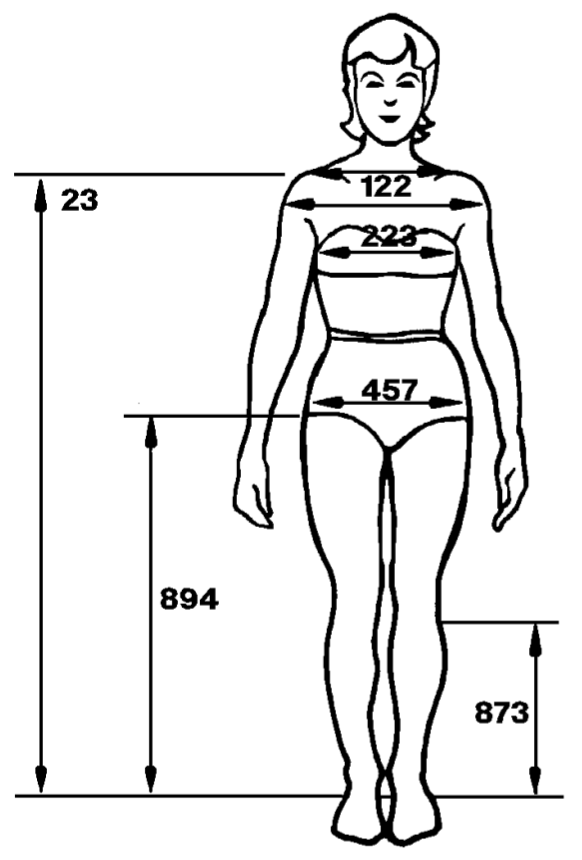
\includegraphics[width = \textwidth]{image_female}
		\caption{\textit{``Body Size of the 40-Year-Old Japanese Female for Year 2000 in One Gravity Conditions.''} \textbf{23} $\widehat{=}$ 1,271m.}
		\label{fig:image_female}
	\end{subfigure}
	\hspace{60pt}
	\begin{subfigure}[b]{0.3\textwidth}
		\centering
		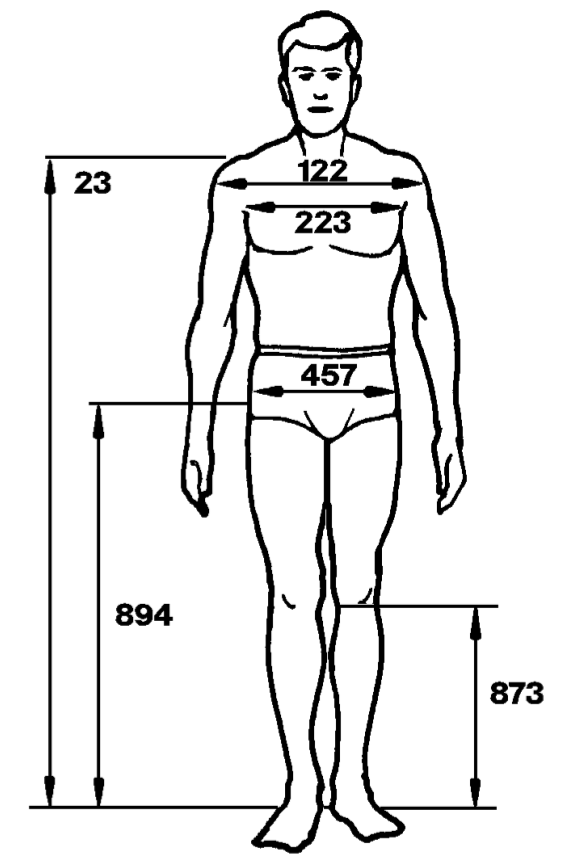
\includegraphics[width = \textwidth]{image_male}
		\caption{\textit{``Body Size of the 40-Year-Old American Male for Year 2000 in One Gravity Conditions.''} \textbf{23} $\widehat{=}$ 1,476m.}
		\label{fig:image_male}
	\end{subfigure}
	\caption{Anthropometric dimensional data for the american female and male. (Image and caption credit: \cite{Hinker:2007, Adolf:2020})}
	\label{fig:bodies}
\end{figure}
When it is assumed that the SL 2600 is operated at shoulder height, then its antenna is $1,271\mathrm{m}$ above the ground for a female and $1,476\mathrm{m}$ above the ground for a male safety officer \cite{Hinker:2007, Adolf:2020}. For the link budget estimation $h_\mathrm{SFTY} = 1,271\mathrm{m}$ is used.